With the 'sndfile' plugin it is possible to play back the content of a
sound file at a given time, or triggered via OSC messages.

\input{tabsndfile.tex}

\paragraph{Multi-channel sound files}
%
If the plugin receives multiple channels (e.g., when used in a
receiver or a diffuse sound field), all channels starting at channel
number \attr{channel} will be returned. If the file does not contain a
sufficient number of channels, silence will be returned for all
channels not available in the sound file.

\paragraph{Calibration of levels}
%
In the level mode ``rms'', the RMS value of the first used channel
will be used for adjusting the level, i.e., all channels will be
scaled with the same value such that the first channel has the
level \attr{level}.
\begin{itemize}
\item Level mode ``rms'' scales the signal so the RMS of the first channel corresponds to \attr{level}.

\item Level mode ``peak'' scales the signal so the peak over all channels corresponds to \attr{level}.

\item Level mode ``calib'' scales the signal by \attr{level} minus 93.979~dB.
\end{itemize}
93.979~dB corresponds internally to a full-scale signal.

\paragraph{Temporal alignment}
%
All times are defined relative to the object time of the parent object
of the sound file plugin. In most cases this is equivalent to the
session time, however, it may be changed with the \attr{start}
attribute of the objects in scenes. If the parent object is not within
a scene (e.g., a 'route' module), the session time is used.

See also Figure \ref{fig:ap_sndfile} for more details on the time and position conventions.

\begin{figure}[htb]
    \centering
    \fbox{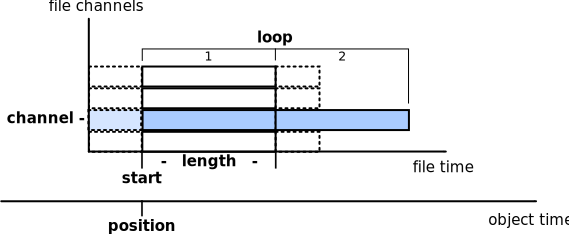
\includegraphics[width=\textwidth]{ap_sndfile}}
    \caption{Explanation of {\tt sndfile} audio plugin attributes.}
    \label{fig:ap_sndfile}
\end{figure}

